% Version on April 8, 2013
% Submitted to jspi on April 8, 2013
%\documentstyle[12pt]{article}
\documentclass[12pt]{article}
\usepackage{latexsym, epsfig, amssymb, amsmath, amsthm, graphicx, mathrsfs}
\usepackage{color}
\usepackage{natbib}
 \textheight=8.0truein
 \textwidth=5.3truein
 \topmargin -0.2in
 \oddsidemargin 0.5in
 \def\nh{\noindent\hangindent=0.45truecm\hangafter=1}
 \def\sqr#1#2{{\vcenter{\hrule height.#2pt \hbox{\vrule width.#2pt
 height#2pt \kern#1pt \vrule width.#2pt} \hrule height.#2pt}}}
 \def\square{\mathchoice\sqr34\sqr34\sqr{2.1}3\sqr{1.5}3}
 \newcommand{\btheta}{{\mbox{\boldmath$\theta$}}}
 \newcommand{\balpha}{{\mbox{\boldmath$\alpha$}}}
 \newcommand{\bomega}{{\mbox{\boldmath$\omega$}}}
 \newcommand{\bg}{{\mbox{\boldmath$g$}}}
 \newcommand{\meta}{{\mbox{\boldmath$\eta$}}}
 \newcommand{\bmu}{{\mbox{\boldmath$\mu$}}}
 \newcommand{\bM}{{\mbox{\boldmath$M$}}}
 %\newtheorem{defi}{\sc Definition}[section]
%\newtheorem{theo}{\sc Theorem}[section]
%\newtheorem{lemm}{\sc Lemma}[section]
%\newtheorem{prop}{\sc Proposition}[section]
%\newtheorem{coll}{\sc Corollary}[section]
%\newtheorem{rema}{\sc Remark}[section]
%\newtheorem{theo1}{\sc Theorem}[section]
%\newtheorem{lemm1}{\sc Lemma }[section]
 \newtheorem{defi}{\sc Definition}
\newtheorem{theo}{\sc Theorem}
\newtheorem{lemm}{\sc Lemma}
\newtheorem{prop}{\sc Proposition}
\newtheorem{coll}{\sc Corollary}
\newtheorem{rema}{\sc Remark}
\newtheorem{theo1}{\sc Theorem}
\newtheorem{lemm1}{\sc Lemma }
\newcommand{\tod}{\stackrel{d}{\longrightarrow}}
\newcommand{\tow}{\stackrel{{\cal{W}}}{\longrightarrow}}
\newcommand{\mstackit}[2]{\mbox{\raisebox{-1.1ex}{$\stackrel{{\textstyle{#1}}}{\
 scriptstyle{#2}}$}}\mbox{}}
  \newcommand{\herefig}[2]{\leavevmode
                           \epsfxsize=#1
                           \epsffile{#2} }
\renewcommand{\theequation}{\arabic{section}.\arabic{equation}}
\renewcommand{\baselinestretch}{1.25}
\makeatletter
 %\@addtoreset{equation}{section}
  \makeatother
  \def\ssc{\sscriptstyle}
  \def\txs{\textstyle}
   \def\half{\txs{1\over 2}}
  \def\sn{\smallskip}
  \def\mn{\medskip}
  \def\ssn{\smallskip\noindent}
  \def\msn{\medskip\noindent}
  \def\bsn{\noindent}
  \def\nshs{\noalign{\smallskip\hrule\smallskip}}
  \def\ns{\noalign{\smallskip}}
  \def\nsh{\noalign{\smallskip\hrule}}
  \def\nhs{\noalign{\hrule\smallskip}}
  \def\po{\phantom1}
  \def\poo{\phantom{11}}
  \def\pooo{\phantom{111}}
  \font\er=cmr8
\def\be{\begin{equation}}
  \def\ee{\end{equation}}
  \def\nn{\nonumber}
  \def\bea{\begin{eqnarray}}
  \def\eea{\end{eqnarray}}
  \def\bw{\bar{w}}
  \pagenumbering{arabic}

\def\vv{1.3}

\begin{document}

\begin{center}
 {\bf \large Confidence intervals for probability
density functions under strong mixing samples }
\end{center}

\bigskip

\begin{center}
Qingzhu Lei \ \ \  Yongsong Qin
\footnote{Corresponding author. Tel: +86-773-5851556

\ \ \  Email address: ysqin@gxnu.edu.cn (Y. Qin)}
\bigskip

%{\small  $^{a}$Department of Mathematics, Zhejiang  Normal University\\
%Jinhua, Zhejiang 321004, China}

{\small  Department of Mathematics, Guangxi Normal University\\
Guilin, Guangxi 541004, China}
\bigskip
\end{center}



 \noindent
{\bf Abstract }  It is shown that the empirical likelihood (EL) ratio statistic for a probability density function is asymptotically
$\chi^2$-type distributed under a strong mixing sample, which is used to obtain an EL-based confidence interval for the  probability density function.
Results of a simulation study on the finite sample performance of the confidence
interval are reported.


\noindent {\it Keywords:}  probability density function;
empirical likelihood; $\alpha$-mixing; confidence interval


\noindent {\it Running title:} Confidence intervals for probability density functions

\noindent AMS 2000 subject classification: Primary 62G05\ \ \  secondary
62E20


\newpage

\setcounter{section}{1}
\setcounter{equation}{0}

 \noindent
{\bf 1. Introduction}
\bigskip

Let $\{\eta_i, 1\geq 1\}$ be a random variable sequence and
${\cal{F}}^t_s$ denote the $\sigma$-algebra generated by $\{\eta_i,
s\leq i\leq t\}$ for $s\leq t$.  Random variables $\{\eta_i, 1\geq
1\}$ are said to be strongly mixing or $\alpha$-mixing (e. g. Rosenblatt, 1956), if
\[
\alpha(n)=\sup_{k\geq 1}\sup_{ A\in {\cal{F}}^k_1 , B\in
{\cal{F}}^{\infty}_{k+n}}|P(AB)-P(A)P(B)| \to 0
\]
as $n\to \infty$, where $\alpha(n)$ is called $\alpha$-mixing coefficient.

The dependence described by $\alpha$-mixing  is the weakest among well-known mixing structures, as it is implied by other types of mixing structures such as the widely used
$\phi$, $\rho$ and $\beta$-mixings; see Doukhan (1994) for a comprehensive discussion on mixing.  Chanda  (1974)  and Gorodetskii  (1977) showed that linear processes are strongly mixing under certain conditions. Withers (1981) further derived an alternative set of conditions for the linear processes to be strongly mixing. Pham and Tran (1985) also studied some sufficient conditions for strongly mixing linear processes. Genon-Catahot et al. (2000) showed that some continuous time diffusion models and stochastic volatility models are strongly mixing as well, which include some most popular models in the pricing theories of financial assets, such as the Black-Scholes pricing theory of options.


Robinson (1983) studied the asymptotic normality
of the kernel estimators of a probability density function (p.d.f.) under $\alpha$-mixing samples. Lu (2001) investigated the asymptotic normality
of the kernel estimators of a p.d.f. under more general dependent samples. However, these results can not be directly used to construct the
confidence intervals for the p.d.f as a variance estimator is required to obtain a confidence interval based on the normal approximation. This estimation of variance is much more involved than independent cases.  Our aim is to construct the empirical likelihood (EL) based confidence intervals for a p.d.f. under $\alpha$-mixing samples without variance estimation.

The EL method to construct confidence intervals, proposed by Owen
(1988, 1990), has many advantages over its counterparts like the
normal-approximation-based method and the bootstrap method (e.g.,
Hall and La Scala 1990; Hall, 1992). Chen (1996) developed the EL
method in construction of a p.d.f. under independent samples.

Kitamura (1997) first proposed  blockwise EL method to construct
confidence intervals for parameters with $\alpha$-mixing samples.  Chen and Wong (2009) developed  blockwise EL method to construct
confidence intervals for quantiles with $\alpha$-mixing samples.  Qin et al. (2011) used the blockwise EL method to construct confidence
intervals for a p.d.f. under negatively associated samples.
Xiong and Lin (2012) demonstrated that the usual EL method can be used to construct confidence intervals for a p.d.f. under associated samples and this method
performs as well as the blockwise EL method. We thus use the usual EL method rather than the blockwise EL method in this paper. The main
 advantage to use the usual EL method is that we do not need to choose the block lengths in constructing the EL ratio statistics and the EL
confidence intervals.
%However, from a theoretical point of view (see Condition A3 below),
%the bandwidth may depend on the block lengthes and the mixing coefficient, which may lead to complexity
%in choosing the optimal bandwidth. Further study in choosing the bandwidth is surely needed in the case of dependent samples,
%which will be left for our future study.


The rest of the paper is organized as follows. The main results of this paper are presented in Section 2.
Results of a simulation study on the finite sample performance of the proposed confidence
intervals are reported in Section 3.
Some lemmas to prove the main results are given in Section 4. The proof of the main results is  presented in
Section 5.

\bigskip
\setcounter{section}{2}
\setcounter{equation}{0}
\noindent {\bf 2. Main results}
\bigskip

Let $X_1,\cdots, X_n$ be a stationary $\alpha$-mixing sample from a
population $X\in R$ and $f(\cdot)$ be the p.d.f. of
$X$. The kernel density estimator of $f(x)$ at a
given $x\in R$ is
\be
f_n(x)=(nh)^{-1}\sum_{i=1}^nK\{h^{-1}(x-X_i)\},
\ee
where $K$ is a kernel function, and $h=h_n$ are bandwidths.

Let $K_h(u)=K(u/h)$ for any $u\in R$, $\theta=f(x)$ at a
given $x\in R$ and $\omega_{ni}=\omega_{ni}(\theta)=h^{-1}K_h(x-X_i)-\theta, 1\leq i\leq n$.
We consider the following EL ratio
 $$R(\theta) = \sup\limits_{p_1, \cdots, p_n}\{\prod_{i=1}^{n}np_i|
 \sum_{i=1}^{n} p_i=1, p_i\geq 0 ,
 \sum_{i=1}^{n} p_i\omega_{ni}(\theta)=0\}.$$
 It is easy to obtain the ($-2$log)  EL ratio statistic
 \be
\ell(\theta)=2\sum_{i=1}^{n} \log \{1+\lambda(\theta)\omega_{ni}(\theta)\},
\label{lambda0}
 \ee
 where $\lambda(\theta)$ is determined by
\be
\sum_{i=1}^{n}
 \frac{\omega_{ni}(\theta)}{1+\lambda(\theta)\omega_{ni}(\theta)}=0.
 \label{lambda}
\ee

 To obtain the asymptotical
distribution of $\ell(\theta)$, we need the following assumptions.

%\noindent {\bf Assumption  }
\smallskip

{\bf Assumptions.}

(A1)  (i) The r.v.s $X_1, X_2, \cdots, X_n$ form a stationary sequence, and let $f$ be the one-dimensional
marginal p.d.f. (with respect to Lebesgue measure).

\ \ (ii) $\{X_i, 1\leq i\leq n\}$ is a $\alpha$-mixing sequence with mixing coefficient $\alpha(\cdot)$.

\ \ (iii) The joint p.d.f.  $f_{1, j}$  of the r.v.s. $X_1, X_{j+1}$ exists and $|f_{1, j}(u, v)-f(u)f(v)|\leq C$
 for all $u, v\in R$ and $j>1$.

 \ \ (iv) $f''$ exists and is bounded in a neighborhood of $x$, and $f(x)>0$.

(A2)     The function $K$ is bounded, has compact support and satisfies $\int K(u)du=1, \int uK(u)=0$ and  $0<\int u^2K(u)du<\infty$.

%\ \ (ii) The derivative $(d/du)K(u) = K'(u)$ exists for all $u \in R$ and is bounded $|K'(u)|\leq C, u \in R$.

(A3)   Let $p=p(n)$ and $q=q(n)$ be positive integers satisfying $p+q\leq n$, and $ k=[n/(p+q)]$, where $[t]$ denotes the integer part of $t$. $p, q$ and $h$ satisfy

\ \ (i) $q/p\to 0, p/n\to 0$,  $ph\to 0, p^2/(nh)\to 0, (1/h)\sum^{\infty}_{s=p}\alpha(s)\to 0, k\alpha(q)\to 0$.

\ \ (ii)  $nh^5\to 0$ as $n\to \infty$.

\smallskip

%{\bf Remark 1. } Let $K(u)=(1-u^2)^2(\sum^r_{j=0}a_ju^j)I(|u|\leq 1)$, where
%$I$ is the indicator function. By putting this kernel into Assumption (A2)(i) and
%solving linear equations to obtain $a_j, 0\leq j\leq r$, we can see that $K$ satisfies Assumption (A2). Specially,  we
%can choose  $K(u)=(15/16)(1-u^2)^2I(|u|\leq 1)$ when $r=2$.

%{\bf Remark 2. } We can  replace Assumption (A1) to (A3) by the
%conditions of Corollary 2.1 in Roussas (2000) in the case of
%$r=1$ or $r=2$.

{\bf Remark 1. }   From A3 (i), it can be shown that $pk/n\to 1, qk/n\to 0, p\to \infty, h\to 0$, $nh\to \infty$ and $(1/h)\sum^{\infty}_{s=q}\alpha(s)\to 0$.
These facts will be used throughout this article. However,
no explicit mentioning will be made.

\smallskip

{\bf Remark 2. } To clearly see the relationship among $p, q$ and $h$, let $C$ be some positive constant, $p=[n^{\beta_1}], q=[n^{\beta_2}]$ and $h=Cn^{-\beta_3}$, where $0<\beta_j<1, j=1, 2, 3$.  Under the assumption that $\alpha (m) \leq C m^{-\tau_0}$ for some constant $\tau_0>2$,
the following conditions (\ref{cona.01}) and (\ref{cona.02}) are sufficient conditions
to ensure Assumption A3 to hold:
\be
 \max  \{ \beta_1, 1/5  \}<\beta_3  <  \min \{  1-2\beta_1, (\tau_0-1)\beta_1 \}, \label{cona.01}
\ee
\be
\beta_1>\max\{ \beta_2, 1-\tau_0\beta_2\}.            \label{cona.02}
\ee
$\beta_3$ in (\ref{cona.01}) can be attained  if we choose $\beta_1$ and $\beta_2$ such that
\be
\max\{  \beta_2, 1-\tau_0\beta_2\}<\beta_1 < 1/3.           \label{cona.03}
\ee
$\beta_1$  in (\ref{cona.03}) can be attained if we choose $\beta_2$ such that
\[
2/(3\tau_0)<\beta_2<1/3.
\]
We note that, in the case of the EL method for quantiles studied in Chen and Wong (2009), it is required that  $\alpha (m) \leq C m^{-\tau_0}$ for some $\tau_0>2$.


\smallskip

Theorem \ref{theo3.1}
shows that $\ell(\theta)$ converges in distribution  to $\chi^2_1$.
%\noindent
\begin{theo}\label{theo3.1}
Suppose Assumptions (A1) to (A3) hold. Then
\[
\ell(\theta)\tod \chi^2_1, \label{lim00.01}
\]
where $\chi^2_1$ is a chi-squared distributed random variable with
one  degree of freedom.
\end{theo}


Let $z_{\alpha}$ satisfy  $P(\chi^2_1\leq z_{\alpha})=1-\alpha$ with $0<\alpha<1$.
It follows from Theorem \ref{theo3.1} that an EL-based confidence interval for $\theta=f(x)$ with asymptotically correct
coverage probability $1-\alpha$ can be constructed as
\be
\{ \theta: \ell(\theta)\leq z_{\alpha} \}. \label{elci}
\ee


\bigskip
\setcounter{section}{3}
\setcounter{equation}{0}
 \noindent
{\bf 3. Simulation results}
\bigskip


%For comparison purpose, we carry out simulation for both normal approximation and EL based confidence intervals.
We denote the EL-based confidence interval (CI) for $\theta=f(x)$ given by (\ref{elci})  as ELCI. On the other hand,
the normal approximation-based confidence interval for $\theta=f(x)$ derived from Lemma \ref{lemm3.1} shown in (\ref{naci}) is denoted as NACI.
\be
[f_n(x)-\hat{\sigma}(x)u_{\alpha}/(nh)^{1/2},     f_n(x)+\hat{\sigma}(x)u_{\alpha}/(nh)^{1/2} ],  \label{naci}
\ee
where $\hat{\sigma}^2(x)=(n^{-1}h)\sum^{n}_{i=1}\omega^2_{ni}(f_n(x))$ and $P(|N(0, 1)|\leq u_{\alpha})=1-\alpha$.


We conducted a small simulation study  to compare the finite sample performances of the confidence intervals ELCI and NACI.
In the simulations, we considered two AR models:
\be
X_t=(1/2)X_{t-1}+\epsilon_t,     \label{model1}
\ee
and
\be
X_t=(3/4)X_{t-1}-(1/8)X_{t-2}+\epsilon_t,  \label{model2}
\ee
where $\{\epsilon_t\}$ is an i.i.d. $N(0, 1)$ random variable sequence. We can see that both models are stationary and $\alpha$-mixing with $X_1\sim N(0, 4/3)$
for model (\ref{model1}) and  $X_1\sim N(0, 32/17)$
for model (\ref{model2}).


We generated $1,000$ random samples of  data $\{X_{i}, \ i=1,
\cdots, n\}$ for $n=100, 150, 200$ and $250$ from above  models.
 In the simulation,  we took $h=4n^{-1/5}/log n$ and
$K$ was chosen as
\[
K(u)=(15/ 16)(1-u^2)^2I(|u|\leq 1).
\]
Let $f$ be the p.d.f. of $X_1$. For nominal confidence level $1-\alpha=0.95$, using the simulated samples, we evaluated the
coverage probabilities (CP) and average lengthes (AL)
of ELCI and NACI for $f(x)$ at $x=0$ and $1$. Table 1 reports the simulation results for model (\ref{model1}), while table 2 reports
the simulation results for model (\ref{model2}).

In the simulations, we used bisection method to solve (\ref{lambda}) to obtain $\lambda(\theta)$. For further description of the computation of $\lambda(\theta)$, we refer to Section 3 in Owen (1990). A DELL Workstation PWS650 with 2G main memory, 2.6G CPU and WINDOWS 2000 was used to do the simulations.
Four minutes and fifty seconds were respectively used to obtain  the ELCI and NACI results in Table 1.


It can be seen from
Tables 1 and 2 that
%the coverage probabilities are close to the nominal level, and that
the larger the sample size is, the closer the coverage probability is to the nominal level. The lengths of the
estimated confidence intervals  decrease with increasing sample size. It is seen  that ELCI performs better than NACI
since the associated confidence intervals have higher coverage accuracies and short average lengths.

Further, we plot in Figure \ref{fig1} the true density function $f(x)$ (TRUE),
and the pointwise CI calculated via the two methods (NA \& EL). In Figure \ref{fig2}, we plot the true density function $f(x)$ (TRUE),
the pointwise NACI calculated via the true variance (TNA) and estimated variance (NA).
In Figure \ref{fig3}, we plot the coverage probabilities (CP) and average lengths (AL) of confidence intervals for  $f(0)$ under model (\ref{model1}) via the two methods (EL \& NA) as $h$ varies.

We observe from Figure \ref{fig1} that
ELCI and NACI have similar performances in terms of the length of CI if the estimated variance is used. However, from Figure \ref{fig2}, we can see that the variance is under-estimated. From Figure \ref{fig3}, we can see that ELCI performs better than NACI
in terms of the coverage probabilities as $h$ varies.   These results, shown in Figures 1, 2  \& 3, may imply that the EL method has better performance than the normal approximation method.

We found (in un-reported simulation results) that the simulation outputs were similar (change little) when $h$ was chosen $Cn^{-1/5}/\log n$ with $3\leq C \leq 5$. We also found that the bandwidth had big impact on the performance of the proposed method.

 If we further assume that $f''$ is continuous at $x$, then under Condition A2, it can be shown that
\[
E\{f_n(x)\}-f(x)=(1/2)h^2f''(x)\int u^2K(u)du+o(h^2).
\]
Combining with Lemma \ref{lemm4.04}, we have
\[
E\{f_n(x)-f(x)\}^2=(nh)^{-1}\sigma^2(x)+(1/4)h^4\{f''(x)\int u^2K(u)du\}^2+o(h^2)+o((nh)^{-1}),
\]
where $\sigma^2(x)=f(x)\int K^2(u)du$. The choice of $h$ which minimizes the main order term of $E\{f_n(x)-f(x)\}^2$ is
\[
h=\sigma^2(x)\{f''(x)\int u^2K(u)du\}^{-2}n^{-1/5}.
\]
By the plug-in approach, the choice of $h$ by the MSE criterion is
\[
\hat{h}=\hat{\sigma}^2(x)\{\hat{f}''(x)\int u^2K(u)du\}^{-2}n^{-1/5},
\]
where $\hat{\sigma}^2(x)=(n^{-1}h)\sum^{n}_{i=1}\omega^2_{ni}(f_n(x))$  and $\hat{f}''(x)$ is a suitable estimator of $f''(x)$ (e. g. Singh, 1977).

We noticed that the choice of $h$ by above
 mean square error (MSE) criterion did not perform well in simulations.
The choice of the bandwidth is an important issue. There is no satisfactory approach available now. Further study in choosing the bandwidth is surely needed in the case of dependent samples. To choose an optimal bandwidth, one may need to derive an Edgeworth expansion for the EL statistic as Chen (1996), which is left for our future study.





\bigskip

\noindent

\begin{center}

 Table 1. \ Coverage probabilities (CP) and average lengths (AL) of confidence intervals for  $f(x)$ under model (\ref{model1}) at $x=0$ and $1$
\end{center}


\begin{center}
\begin{tabular}{ccccccc}
\hline  &   & \multicolumn{2}{c}{CP}
     &&\multicolumn{2}{c}{AL}\\
\cline{3-4} \cline{6-7}
$x$ & $n$ &  ELCI   & NACI   && ELCI  & NACI  \\
\cline{3-4} \cline{6-7}
 $x=0$ & $100$  & 0.931  & 0.911 & &  0.2919& 0.2944 \\
          & $150$  &  0.933 & 0.926 & & 0.2693 & 0.2694 \\
          & $200$  &  0.934  & 0.927& & 0.2599 & 0.2701 \\
          & $250$  &  0.937 & 0.930  & & 0.2344& 0.2345\\
$x=1$ & $100$  & 0.914  & 0.896 & &  0.2531& 0.2542\\
          & $150$  &  0.922 & 0.916 & & 0.2261 & 0.2353 \\
          & $200$  &  0.932  & 0.921 & & 0.2109& 0.2203 \\
          & $250$  &  0.936 & 0.928  & & 0.1976& 0.2071\\
 \hline
\end{tabular}
\end{center}


\bigskip

\noindent

\begin{center}

 Table 2. \ Coverage probabilities (CP) and average lengths (AL) of confidence intervals for  $f(x)$ under model (\ref{model2}) at $x=0$ and $1$
\end{center}


\begin{center}
\begin{tabular}{ccccccc}
\hline  &   & \multicolumn{2}{c}{CP}
     &&\multicolumn{2}{c}{AL}\\
\cline{3-4} \cline{6-7}
$x$ & $n$ &  ELCI   & NACI   && ELCI  & NACI  \\
\cline{3-4} \cline{6-7}
 $x=0$ & $100$  & 0.926  & 0.912 & &  0.2794& 0.2894 \\
          & $150$  &  0.931 & 0.927 & & 0.2510 & 0.2608 \\
          & $200$  &  0.935  & 0.930 & & 0.2329& 0.2428 \\
          & $250$  &  0.936 & 0.931  & & 0.2185& 0.2284\\
$x=1$ & $100$  & 0.906  & 0.886 & &  0.2473& 0.2562 \\
          & $150$  &  0.913 & 0.896& & 0.2224 & 0.2315 \\
          & $200$  &  0.915  & 0.903 & & 0.2043& 0.2236 \\
          & $250$  &  0.922 & 0.916  & & 0.1934& 0.2029\\
 \hline
\end{tabular}
\end{center}


\renewcommand{\baselinestretch}{\vv}

\begin{figure}[htbp]
\begin{tabular}{cc}
\includegraphics[width=0.90\textwidth]{fig1.eps}  %& \includegraphics[width=0.45\textwidth]{fig2.eps}
\end{tabular}
\caption{ The true density function $f(x)$ (TRUE),
the pointwise CI calculated via the two methods (EL \& NA) with $n=250$. (a) is for model (\ref{model1}) and (b) is for model (\ref{model2}).   }
    \label{fig1}
\end{figure}


\renewcommand{\baselinestretch}{\vv}

\begin{figure}[htbp]
\begin{tabular}{cc}
\includegraphics[width=0.90\textwidth]{fig2.eps}  % & \includegraphics[width=0.45\textwidth]{fig4.eps}
\end{tabular}
\caption{ The true density function $f(x)$ (TRUE),
the pointwise NACI calculated via the true variance (TNA) and estimated variance (NA) with $n=250$. (a) is for model (\ref{model1}) and (b) is for model (\ref{model2}). }
    \label{fig2}
\end{figure}

\renewcommand{\baselinestretch}{\vv}


\begin{figure}[htbp]
\begin{tabular}{cc}
\includegraphics[width=0.90\textwidth]{bandwidth1.eps}  %& \includegraphics[width=0.45\textwidth]{fig2.eps}
\end{tabular}
\caption{ Coverage probabilities (CP) and average lengths (AL) of confidence intervals for  $f(0)$ under model (\ref{model1})  via the two methods (EL \& NA) with $n=100$ as $h$ varies. (a) is for CP and (b) is for AL.   }
    \label{fig3}
\end{figure}


%\renewcommand{\baselinestretch}{\vv}

%\begin{figure}[htbp]
%\begin{tabular}{cc}
%\includegraphics[width=0.90\textwidth]{bandwidth2.eps}  % & \includegraphics[width=0.45\textwidth]{fig4.eps}
%\end{tabular}
%\caption{ The true density function $f(x)$ (TRUE),
%the pointwise NACI calculated via the true variance (TNA) and estimated variance (NA) with $n=250$. (a) is for model (\ref{model1}) and (b) is for model (\ref{model2}). }
%    \label{fig4}
%\end{figure}



\bigskip
\setcounter{section}{4}
\setcounter{equation}{0}
 \noindent
{\bf 4. Lemmas}
\bigskip

We use $C$ to denote a positive constant independent of $n$, which
may take a different value for each appearance.
For any integer $s\geq 1$ and random variable $\xi$ with  $E|\xi|^s<\infty$, denote $||\xi||_s=\{E|\xi|^s\}^{1/s}$.   To prove our main results,
we need following lemmas.

\begin{lemm}\label{lemm4.01}
Let $\{\eta_i, i\geq 1\}$ be a $\alpha$-mixing process and
${\cal{F}}^t_s$ denote the $\sigma$-algebra generated by $\{\eta_i,
s\leq i\leq t\}$ for $s\leq t$. Suppose that $\xi$ and $\eta$ are
random variables which are ${\cal{F}}^k_1$ and ${\cal{F}}^{\infty}_{k+m}$ measurable, respectively, and
that $||\xi||_{p_1}<\infty, ||\eta||_{q_1}< \infty$, where $p_1, q_1>1, p_1^{-1}+q_1^{-1}<1$. Then,
\[
|E(\xi\eta)-E(\xi)E(\eta)|\leq 10\{\alpha(m)\}^{1-p_1^{-1}-q_1^{-1}}||\xi||_{p_1}||\eta||_{q_1}.
\]
If $\xi$ and $\eta$ are bounded
random variables, then
\[
|E(\xi\eta)-E(\xi)E(\eta)|\leq C\alpha(m),
\]
were $C$ is a positive constant.
\end{lemm}

{ \bf Proof. } See Lemma 1 in Deo (1973).


\begin{lemm}\label{lemm4.02}
Let $\{\eta_i, i\geq 1\}$ be a $\alpha$-mixing process and
${\cal{F}}^t_s$ denote the $\sigma$-algebra generated by $\{\eta_i,
s\leq i\leq t\}$ for $s\leq t$. Suppose that  $\{\xi_i, 1\leq i\leq n\}$  are  ${\cal{F}}^{j_1}_{i_1}, \cdots,
{\cal{F}}^{j_n}_{i_n}$ measurable, respectively with $1\leq i_1<j_1<i_2\cdots<j_n, i_{l+1}-j_l\geq m$, and $|\xi_l|\leq 1$ for
$l=1, \cdots, n$. Then,
\be
|E(\prod^n_{l=1}\xi_l)-\prod^n_{l=1}E(\xi_l)|\leq 16(n-1)\alpha(m). \label{0.0}
\ee
\end{lemm}

{ \bf Proof. } See Lemma 1.1 in Volkonkii and Rozanov (1959).  Note that (\ref{0.0}) is also true for complex random variables
$\{\xi_i, 1\leq i\leq n\}$ with $|a|$ replaced by the norm of a complex number $a$.


\smallskip

\begin{lemm}\label{lemm4.04}
Under the conditions of Theorem \ref{theo3.1}, as $n\to \infty$,
\be
(nh)Var(f_n(x))=\sigma^2(x)+o(1), \label{lem06.04.1}
\ee
\be
\sqrt{nh}\{f_n(x)-Ef_n(x)\}\tod N(0, \sigma^2(x)) \label{lem06.04.2},
\ee
where $\sigma^2(x)=f(x)\int K^2(u)du$.
\end{lemm}

{\bf Proof. } In the sequel, we employ the small-block and large-block arguments to prove Lemma \ref{lemm4.04}, where $p, q$ and $k$ are given in condition A3. Let $Z_{ni}=K_h(x-X_i)-EK_h(x-X_i), 1\leq i\leq n$, and
\[
S_n=\sqrt{nh}\{f_n(x)-Ef_n(x)\}.
\]
Then $S_n$ can be split as
$S_n=S'_n+S''_n+S'''_n$, where
$S'_n=\sum_{m=1}^ke_{nm}$,
$S''_n=\sum_{m=1}^ke'_{nm}$ and
$S'''_n=e'_{n, k+1}$,
with
$e_{nm}={1\over \sqrt{nh}}\sum_{i=r_m}^{r_m+p-1}Z_{ni},
e'_{nm}={1\over \sqrt{nh}}\sum_{i=l_m}^{l_m+q-1}Z_{ni},
e'_{n, k+1}={1\over \sqrt{nh}}\sum_{i=k(p+q)+1}^nZ_{ni},
r_m=(m-1)(p+q)+1,l_m=(m-1)(p+q)+p+1, m=1,\cdots, k$.


 (\ref{lem06.04.2}) follows if we can verify
 \be S'_n
\tod N(0, \sigma^2(x)),\label{s}
\ee
\be
S''_n=o_p(1),\label{ss}
\ee
and
\be
S'''_n=o_p(1).\label{sss}
\ee

As a preparation, we first show that
\be
Var(S'_n)=\sigma^2(x)+o(1).\label{sss.0}
\ee
From Lemma 3.1 in Roussas (2000), using conditions A1 (i), A1 (iii), A1 (iv), A2, $kp/n\to 1$ and $ph\to 0$, we can see that
\[
{k\over nh}\sum_{1\leq i<j\leq p}  |Cov(Z_{ni}, Z_{nj})|\leq {Ckp^2h\over n}\to 0,
\]
and
\be
\sum_{m=1}^k Var(e_{nm})={kp\over nh} Var(Z_{n1})+{2k\over nh}\sum_{1\leq i<j\leq p}  Cov(Z_{ni}, Z_{nj}) \to \sigma^2(x).  \label{sss.0.1}
\ee
By stationarity and the proof of Lemma 3.2 (ii) in Roussas (2000), it can be shown that
\bea
&& \sum_{1\leq i<j\leq k}|Cov(e_{ni}, e_{nj})| = \sum^{k-1}_{l=1}(k-l)|Cov(e_{n1}, e_{n, l+1})|\nn\\
&&\leq k\sum^{k-1}_{l=1}|Cov(e_{n1}, e_{n, l+1})|
\leq  {kp\over nh}\sum^{k-1}_{l=1} \sum_{s=l(p+q)-p}^{l(p+q)+p}|Cov(Z_{n1}, Z_{n, s+1})|.\nn
\eea
It follows, from Lemma \ref{lemm4.01}, using conditions A3 (i), that
\be
 \sum_{1\leq i<j\leq k}Cov(e_{ni}, e_{nj}) \leq  {Ckp\over nh} \sum^{\infty}_{s=q}  \alpha (s) \to 0.
 \label{sss.0.2}
\ee
(\ref{sss.0}) follows from  (\ref{sss.0.1}) and (\ref{sss.0.2}).

Similarly, we have
\bea
\sum_{m=1}^k Var(e'_{nm}) &=& {kq\over nh} Var(Z_{n1})+{2k\over nh}\sum_{1\leq i<j\leq q}  Cov(Z_{ni}, Z_{nj})\nn\\
& \leq &  {Ckq\over n} + {Ckq^2h\over n}\to 0, \label{uselater1}
\eea
and
\bea
&& \sum_{1\leq i<j\leq k}|Cov(e'_{ni}, e'_{nj})| = \sum^{k-1}_{l=1}(k-l)|Cov(e'_{n1}, e'_{n, l+1})|\nn\\
&&\leq k\sum^{k-1}_{l=1}|Cov(e'_{n1}, e'_{n, l+1})|
\leq  {kq\over nh} \sum^{k-1}_{l=1} \sum_{r=l(p+q)-(q-1)}^{l(p+q)+(q-1)}|Cov(Z_{n1}, Z_{n, r+1})|.\nn
\eea
It follows that
\bea
 E(S''_n)^2
 & \leq & {Ckq\over n} + {Ckq^2h\over n}  +{Ckq\over nh} \sum^{\infty}_{s=p}  \alpha(s) \to 0, \label{ss.1}
\eea
which implies (\ref{ss}).

We can also show that
\be
 E(S'''_n)^2\leq  {C\{n-k(p+q)\}\over n} + {C\{n-k(p+q)\}^2h\over n}
 \rightarrow 0, \label{sss.1}
\ee
which leads to  (\ref{sss}).

We now prove (\ref{s}). From Lemma \ref{lemm4.02}, we have
\be
\left| Ee^{it\sum^k_{m=1}e_{nm}}-\prod^k_{m=1}Ee^{ite_{nm}}\right|\leq C(k-1)\alpha (q) \to 0, \label{s.1}
\ee
which implies that $\{e_{nm}, 1\leq m\leq k\}$ are asymptotically independent.
Let
\[
X_{nm}=\frac{e_{nm}}{\tau_n},~~~\tau_n^2=\sum_{m=1}^{k}Var(e_{nm}).
\]
From $|X_{n1}|\leq Cp/\sqrt{nh}\tau_n$, a.s.,  $Var(X_{n1})=Var(e_{n1})/\tau_n^2=1/k$, we have,
for every $\varepsilon>0$,
\[
\sum_{m=1}^{k}EX_{nm}^2I_{\{|X_{n1}|\geq\varepsilon\}}
\leq\frac{Cp^2k}{nh\tau^2_n}P(|X_{n1}|\geq\varepsilon)
\leq\frac{Cp^2k}{n\tau^2_n}\frac{Var(X_{n1})}{\varepsilon^2}
=\frac{C}{\varepsilon^2\tau^2_n}\frac{p^2}{nh}\rightarrow 0,
\]
where we have used the facts that $\tau^2_n \to \sigma^2(x)$ by (\ref{sss.0.1}) and $p^2/(nh) \to 0$ by assumption.
By the Feller-Lindeberg central limit theorem, we have (\ref{s}).

From (\ref{s}), (\ref{ss}), (\ref{sss}) and the Cramer-Wold theorem, we obtain (\ref{lem06.04.2}).
(\ref{lem06.04.1}) follows from  (\ref{sss.0}),  (\ref{ss.1}) and  (\ref{sss.1}). The proof of Lemma \ref{lemm4.04} is thus complete.

\smallskip

\begin{lemm}\label{lemm3.1}
Under the conditions of Theorem \ref{theo3.1}, as $n\to \infty$, \be
\omega_{n}=\max_{1\leq i\leq n}|\omega_{ni}(\theta)|\leq C
h^{-1}, a. s.,   \label{lemm3.1.1} \ee \be
\sqrt{n^{-1}h}\sum^{n}_{i=1}\omega_{ni}(\theta)\tod N(0,
\sigma^2(x)),  \label{lemm3.1.2} \ee \be
(n^{-1}h)\sum^{n}_{i=1}\omega^2_{ni}(\theta)=\sigma^2(x)+o_p(1),
\label{lemm3.1.3} \ee
 \be
(n^{-1}h)^{3/2}\sum^{n}_{i=1}|\omega_{ni}(\theta)|^3=o_p(1),  \label{lemm3.1.4}
\ee
where $\sigma^2(x)=f(x)\int K^2(u)du$.
\end{lemm}

{\bf Proof. } (\ref{lemm3.1.1}) follows from $|K|\leq C$, $q\leq cp$ and $n-k(p+q)\leq Cp$. Observe that
\[
\sqrt{n^{-1}h}\sum^{2k+1}_{i=1}\omega_{ni}(\theta)
=\sqrt{nh}\{f_n(x)-Ef_n(x)\}+\sqrt{nh}\{Ef_n(x)-f(x)\}.  \label{lemm3.1.2.1}
\]
Condition A3(ii) and standard arguments in the kernel estimation of a p.d.f.  (e.g. Singh, 1977) leads to
\[
\sqrt{nh}\{Ef_n(x)-f(x)\}=\sqrt{nh}O(h^2)=\sqrt{nh^{5}}O(1)=o(1). \label{lemm3.1.2.2}
\]
Combining with Lemma \ref{lemm4.04}, we obtain (\ref{lemm3.1.2}).

We now prove (\ref{lemm3.1.3}). Write
\be
 (n^{-1}h)  \sum^{n}_{i=1}\omega^2_{ni}(\theta)={1\over nh}\sum^n_{i=1}K^2_h(x-X_i)-2hf(x)f_n(x)+hf^2(x). \label{lemm3.1.3.1}
\ee
Note that $nh\to \infty$ from the condition $p^2/(nh)\to 0$. From $nh\to \infty$ and (\ref{lem06.04.1}), we have $Var(f_n(x))\to 0$, i.e.
\be
Var \biggl ( (nh)^{-1}\sum^n_{i=1}K_h(x-X_i) \biggr )\to 0. \label{lemm3.1.3.2}
\ee
In the same way, one can show that
\be
Var \biggl ( (nh)^{-1}\sum^n_{i=1}K^2_h(x-X_i) \biggr )\to 0. \label{lemm3.1.3.3}
\ee
From stationarity, (\ref{lemm3.1.3.2}) and  (\ref{lemm3.1.3.3}), we have
\[
 (nh)^{-1}\sum^n_{i=1}K^j_h(x-X_i)=h^{-1}EK^j_h(x-X_1)+o_p(1), j=1, 2. \label{lemm3.1.3.4}
\]
Standard arguments in the kernel estimation of a p.d.f. lead to $h^{-1}EK^j_h(x-X_1)=f(x)\int K^j(u)du+o(1), j=1,  2$. It follows that
\be
 (nh)^{-1}\sum^n_{i=1}K^j_h(x-X_i)=f(x)\int K^j(u)du+o_p(1), j=1, 2. \label{lemm3.1.3.4}
\ee
(\ref{lemm3.1.3.1}), (\ref{lemm3.1.3.4}) and $h\to 0$ imply (\ref{lemm3.1.3}).

We now prove (\ref{lemm3.1.4}). By $C_r$-inequality, we have
\[
(n^{-1}h)^{3/2}\sum^{n}_{i=1}|\omega_{ni}(\theta)|^3\leq C\{(nh)^{-1/2}(nh)^{-1}\sum^{n}_{i=1}|K^3_h(x-X_i)|+n^{-1/2}h^{3/2}f^3(x)\}.
\]
Similar to the proof of (\ref{lemm3.1.3.4}), we can see that
\[
(nh)^{-1}\sum^{n}_{i=1}|K^3_h(x-X_i)|=f(x)\int |K(u)|^3du+o_p(1).
\]
We thus have (\ref{lemm3.1.4}). The prove of Lemma \ref{lemm3.1} is complete.

\bigskip
\setcounter{section}{5}
\setcounter{equation}{0}
 \noindent
{\bf 5. Proof of Theorem \ref{theo3.1} }
\bigskip

Put
\[
\overline{\omega}=(n^{-1}h)^{1/2}\sum_{i=1}^{n}
\omega_{ni}(\theta),
S=(n^{-1}h)\sum_{i=1}^{n}\omega_{ni}^2(\theta).
\]
From (\ref{lambda}), we have
\[
\sum_{i=1}^{n}\omega_{ni}(\theta)-\lambda(\theta)\sum_{i=1}^{n}
{\omega_{ni}^2(\theta)\over 1+\lambda(\theta)
\omega_{ni}(\theta)}=0.
\]
It follows that
\be
|\sum_{i=1}^{n}\omega_{ni}(\theta)|\geq
{|\lambda(\theta)|\over 1+|\lambda(\theta)|
\omega_{n}}\sum_{i=1}^{n}\omega_{ni}^2(\theta),
\label{theo3.1.10}
\ee
where $\omega_{n}=\max\limits_{1\leq i \leq n} |\omega_{ni}(\theta)|$. From Lemma \ref{lemm3.1}, we have
\[
{|\lambda(\theta)|\over 1+|\lambda(\theta)| \omega_{n}}=O_p((h/n)^{1/2}),
\]
which implies
\be
\lambda(\theta)=O_p((h/n)^{1/2}), \label{proof3.1.1}
\ee
where we have used the facts that $\omega_{n}=O_p(h^{-1})$ and $nh\to \infty$. Let $\gamma_i=\lambda(\theta)
\omega_{ni}(\theta), 1\leq i\leq n$.
Then
\be
\max_{1\leq i \leq
n}|\gamma_i|=O_p((h/n)^{1/2})O_p(h^{-1})=O_p((nh)^{-1/2})=o_p(1). \label{proof3.1.2}
 \ee

Using (\ref{lambda})  again, we have
\begin{eqnarray*}
0 & = & \sum_{i=1}^{n}{\omega_{ni}(\theta)\over 1+\lambda(\theta) \omega_{ni}(\theta)}\\
&=& (n^{-1}h)^{-1/2}\overline{\omega}- (n^{-1}h)^{-1}\lambda(\theta)S+
\sum_{j=1}^{n}\frac{\omega_{ni}(\theta)\gamma_i^2}{1+\gamma_i}.
\end{eqnarray*}
From Lemma \ref{lemm3.1}, (\ref{proof3.1.1}) and (\ref{proof3.1.2}), the final term has the norm bounded by
$$
\sum_{i=1}^{n}\frac{|\omega_{ni}(\theta)|^3|\lambda(\theta)|^2}{|1+\gamma_i|}=o_p((n^{-1}h)^{-1/2}).$$
Therefore, from Lemma \ref{lemm3.1}, we may write \be
\lambda(\theta)=(n^{-1}h)^{1/2}S^{-1}\overline{\omega}+\tau,
\label{proof3.1.3} \ee where \be \tau=o_p((n^{-1}h)^{1/2}).
\label{proof3.1.4} \ee By (\ref{proof3.1.2}) we may expand
$\log(1+\gamma_i)=\gamma_i-\gamma_i^2/2+u_i$ where, for some
finite $B>0,$
$$P(|u_i|\leq B|\gamma_i|^3, 1\leq i \leq n)\rightarrow 1, as ~n\rightarrow \infty.$$
Therefore, from (\ref{lambda0}), (\ref{proof3.1.3}), (\ref{proof3.1.4}) and Taylor expansion, we have
\begin{eqnarray*}
\ell(\theta)& = & 2\sum_{i=1}^{n} \log(
1+\gamma_i)=2\sum_{i=1}^{n}
\gamma_i-\sum_{i=1}^{n}\gamma_i^2+2\sum_{i=1}^{n}u_i\\
&=&  S^{-1}(\overline{\omega})^2
- (n^{-1}h)^{-1}\tau^2S+2\sum_{i=1}^{n}u_i.
\end{eqnarray*}
From  (\ref{proof3.1.4}) and Lemma \ref{lemm3.1}, we obtain that
\[(n^{-1}h)^{-1}\tau^2S=(n^{-1}h)^{-1}o_p((n^{-1}h))O_p(1)=o_p(1),\]
and
$$|\sum_{i=1}^{n}u_i|\leq B |\lambda(\theta)|^3\sum_{i=1}^{n}|\omega_{ni}(\theta)|^3
=O_p((n^{-1}h)^{3/2})o_p((n^{-1}h)^{-3/2})=o_p(1).$$ Therefore, by
the Cramer-Wold's thorem and Lemma \ref{lemm3.1} again, we have
$\ell(\theta)\tod \chi^2_1$, which completes the proof of Theorem
\ref{theo3.1}.




\vskip0.8cm \noindent {\bf Acknowledgements  } The authors are thankful to the referees and the associate editor for their constructive
suggestions. This work was partially supported by the National Natural Science Foundation of China
(11271088, 11361011, 11201088), Guangxi ``Bagui Scholar" Special Project Foundation and the Natural Science Foundation of
Guangxi (2013GXNSFAA019004, 2013GXNSFAA019007, 2013GXNSFBA019001).
%The authors are thankful to the referees for constructive suggestions.

 \vskip0.8cm
\noindent {\bf References}
%\begin{itemize}


\noindent

\nh Chanda, K.C., 1974. Strong mixing properties of linear processes. J. Appl. Probab. 11, 401-408.

\nh   Chen, S. X., 1996. Empirical likelihood confidence intervals for nonparametric density estimation.
Biometrika.  83, 329-341.

\nh Chen, S. X.,  Wong, C. M., 2009.  Smoothed block empirical likelihood for quantiles of
weakly dependent processes.  Statistica Sinica.  19, 71-81.

\nh Deo,  C.  M.,  1973, A  note on empirical processes of strong-mixing sequences. Ann. Probab.
1, 870-875.

\nh Doukhan, P., 1994. Mixing: Properties and Examples. Springer-Verlag: New-York.

\nh Genon-Catahot, V., Jeantheau, T., Laredo, C., 2000. Stochastic volatility models as hidden Markov models and applications. Bernoulli. 6(6), 1051-1079.

\nh Gorodetskii, V.V., 1977. On the strong mixing properties for linear processes. Theory Probab. Appl. 22, 413-441.

%\nh   Hall, P. (1985). Resampling a coverage pattern. Stochastic Process. Appl. 20, 231-246.

\nh  Hall, P., 1992.   The Bootstrap and Edgeworth Expansion.
Springer-Verlag, New York.

\nh  Hall, P., La Scala B., 1990. Methodology and algorithms of empirical likelihood.
Internat. Statist. Rev. 58, 109-127.

\nh   Kitamura, Y., 1997. Empirical likelihood methods with weakly
dependent processes. Ann. Statist.  25, 2084-2102.

%\nh   K\"unsch, H. R. (1989),  The jackknife and the bootstrap for general stationary observations, Ann.
%Statist., 17, 1217-1261.

%\nh  Lahiri, S. (2003),  Resampling Methods for Dependent Data, New York: Springer-Verlag.

\nh Lu, Z. D. , 2001. Asymptotic normality of kernel density estimators under dependence.  Ann.  Inst. Statist.  Math.,  53, 447-468.

\nh  Owen, A. B., 1988.  Empirical likelihood ratio confidence intervals for a single functional.
 Biometrika. 75, 237-249.

\nh  Owen, A. B., 1990. Empirical likelihood ratio confidence regions.
Ann. Statist. 18, 90-120.

%\nh  Politis, D. and Romano, J. P. (1994),  The stationary bootstrap, J. Amer. Statist. Assoc., 89, 1303-1313.

%\item[{[3]}] Owen A B.  Empirical Likelihood.  Chapman \& Hall,  New York (2001)

\nh Pham, T.D., Tran, L.T., 1985. Some strong mixing properties of time series models. Stochastic Process. Appl. 19,  297-303.

\nh Qin, Y., Li, Y.  Lei, Q., 2011. Empirical likelihood for probability density functions
under negatively associated samples. J. Statist. Plann. Inference, 141, 373-381.

\nh Robinson, P. M., 1983. Nonparametric estimators for time series. J. Time Ser. Anal. 4, 185-197.

\nh Rosenblatt, M., 1956. A central limit theorem and a strong mixing condition. Proc. Natl.  Acad.
Sci. U.S.A. 42,  43-47.

\nh  Roussas, G. G., 2000. Asymptotic normality of the
kernel estimate of a probability density function under association.
Statist. Probab. Lett. 50, 1-12.

%\nh Shao, Q. and H. Yu (1996) Weak convergence or weighted empirical processes of dependent
%sequences. The Annals of Probability 24, 2098-2127.

%\nh  Shi, X. Q., 1986.  Bootstrap estimation for the mean of a m-dependent sample.
%Chinese Science Bulletin. 6, 404-407.

\nh  Singh, R. S., 1977. Improvement of some known nonparametric uniformly consistent estimators of
derivatives of a density.  Ann. Statist.  5, 394-399.

\nh Volkonskii, V. A., Rozanov, Y. A., 1959.  Some limit theorems for random functions I.  Theor. Prob.
Appl. 4, 178-197.

\nh Withers, C.S., 1981. Conditions for linear processes to be strong mixing. Z. Wahrsch. Verw. Crebiete. 57, 477-480.

\nh Xiong, X. Lin, Z., 2012. Empirical likelihood inference for probability density functions
under association. J. Statist. Plann. Inference, 141, 373-381. 142, 986-992.

%\end{itemize}
\end{document}
